\chapter{Numerical Background}
%\begin{itemize}
%\item introduction to the boussinesq approximation 
%\item In this section I should introduce the spectral method and the numerical scheme
%\item Dealiasing tests 
%\item  diffusion test
%\item hyperviscosity
%\end{itemize}

In this chapter we discuss the numerical techniques and methods used in this thesis. In this thesis we use the spectral method to numerically solve the linear and nonlinear Navier-Stokes equations. Spectral methods provide a convenient and quick way to compute derivatives of sufficiently well-behaved periodic functions. In evaluating derivatives of smooth periodic functions, spectral methods provide an advantage over other methods of evaluating derivatives, such as finite difference, as the derivatives can be computed to with greater accuracy, often to machine precision, in exchange for only a relatively modest increase in complexity. Specifically, finite difference methods run in $\mathcal{O}(N)$, where $N$ is the number of grid points, but the error tends to be on the order of $\mathcal{O}(N^{-p})$ where $p$ is a small integer. Spectral methods, however, run in $\mathcal{O}(N\log N)$ but the errors are on the order of $\mathcal{O}(N^{-p})$ when the function is $C^{p}$\cite{trefethen_spectral}. A complete overview of spectral methods is beyond the scope of this thesis and we only discuss the key features needed for numerical work. Comprehensive reviews of spectral methods are provided in many books, e.g. Trefethen \cite{trefethen_spectral}, Boyd \cite{boyd2001}, and (spectral method in fluids book). 


\section{Spectral Methods Motivation}
Spectral methods have their origins in the Fourier transform. Let us denote the Fourier transform, $\mathcal{F}$, of $f(x)$ as $\mathcal{F}(f(x)) = \hat{f}(k)$, given by
\begin{align}
\mathcal{F}(f(x)) = \hat{f}(k) = \int_{-\infty}^{\infty}dxe^{-ikx}f(x)\label{fouriertransform},
\end{align}
Now consider the Fourier transform of the derivative $df/dx$. 
\begin{align}
\mathcal{F}\left(\frac{df}{dx}\right)= \int_{-\infty}^{\infty}dxe^{-ikx}\frac{df}{dx}=e^{-ikx}f(x)\bigg|_{-\infty}^{\infty} + ik\int_{-\infty}^{\infty}dxe^{-ikx}f(x)= ik\hat{f}(k),
\end{align}
and thus the Fourier transform of a derivative is just $ik$ times the Fourier transform of $f(x)$. An important assumption here that $f(x)$ vanishes sufficiently quickly at infinity otherwise the $e^{-ikx}f(x)$ term is non-negligible. For most applications of the Fourier transform, but not all,  this assumption is valid. In this thesis, all functions considered will vanish sufficiently so that this term is negligible. For a complete treatment of the conditions when a Fourier transform exists can be found in e.g. (cite some books). With this result in hand, it is easy to show via induction that the Fourier transform of $d^{n}f/dx^{n}$ is $(ik)^{n}\hat{f}(k)$. Hence, once we have the Fourier transform $\hat{f}(k)$, the $n$-th derivative is obtained by computing the inverse Fourier transform
\begin{align}
\frac{d^{n}f}{dx^{n}} = \frac{1}{2\pi} \int_{-\infty}^{\infty}dx e^{ikx}(ik)^{n}\hat{f}(k).\label{inversefouriertransform}
\end{align}

This procedure suggests a method to compute the derivative of a function. Computationally, if we have a way to evaluate $\hat{f}(k)$ from $f(x)$ and $f(x)$ from $\hat{f}(k)$, then the $n$-th derivative is easy to compute via the following algorithm:  
\begin{enumerate} 
\item Compute $\hat{f}(k)$ from $f(x)$
\item Multiply $\hat{f}(k)$ by $(ik)^{n}$ 
\item Invert $(ik)^{n}\hat{f}(k)$ to obtain $f^{(n)}(x)$
\end{enumerate}

We need a method to evaluate the integrals (\ref{fouriertransform}) and (\ref{inversefouriertransform}). One possible avenue would be to apply well known integral quadratures to evaluate these integrals. However, there are more fruitful and better alternatives. The correct avenue to implementing the above algorithm is to consider the discrete analogue of the Fourier transform, the discrete Fourier transform. From the discrete Fourier transform, we discuss the Fast Fourier Transform, which is a fast way to evaluate the discrete Fourier transform.
\section{FFT and Spectral Derivatives} 
Let us now investigate how we can quickly compute the Fourier transform of a function on a computer. In analogue to the Fourier transform, we define the discrete Fourier transform\footnote{Note that there is no universal standard on where to put the factors of $N$ and $2\pi$.} (DFT) on $N$ data points $v_{j}$
\begin{align}
\hat{v}_{k} = \frac{2\pi}{N}\sum_{j=1}^{N} e^{-ikx_{j}}v_{j},\qquad k=-\frac{N}{2}+1,\ldots,\frac{N}{2},\label{dft}
\end{align}
and the inverse discrete Fourier transform (IDFT)  on $N$ data points $\hat{v}_{k}$
\begin{align}
v_{j} = \frac{1}{2\pi}\sum_{k=-N/2+1}^{N/2} e^{ikx_{j}}\hat{v}_{k}, \qquad j=1,\ldots, N.\label{idft}
\end{align}
Here we take $N$ to be even to simplify the formulas, however all results hold for odd $N$ with slight modification. The range of the wavenumbers is from $-N/2+1$ not $-N/2$ due to the $2\pi$ periodicity so wavenumbers $-N/2$ are equivalent to $N/2$ and we do not want to count this wavenumber twice. 

From the definitions of the DFT and inverse DFT, we can see a close analogy to the continuous Fourier and inverse Fourier transforms. It can be shown \cite{trefethen_spectral} that these are the correct discrete analogies. 

First, we need to determine how to sample the function $f(x)$. We assume $f(x)$ to periodic on $0\le x\le 2\pi$. If the domain is different, a simple scaling can transform the periodic domain to this standard interval. To compute the spectral derivative of $f(x)$, we first sample at the points 
\begin{align}
x_{j} = \frac{2\pi j}{N}, j=1,\ldots,N
\end{align}
and set $v_{j}=f(x_{j})$. Now we can compute the DCT from $v_{j}$ giving the coefficients $\hat{v}_{k}$ which is the analogue of $\hat{f}(k)$.  Since this is the analogue of the Fourier transform, we now multiply by $ik$ resulting in the analogue of computing the first derivative. Finally, we compute the inverse DFT from $ik\hat{v}_{k}$ which produces the spectral approximation, $v'_{j}$, to the derivative of the sampled function $f'(x)$ at points $x_{j}$. However, there is some subtleness involved in treating the wavenumber $N/2$, but to make a long story short, we simply set it to $0$ and for details see \cite{trefethen_spectral}. (expand this a bit?)

Despite having a discrete algorithm to compute an analogue of the Fourier transform, our goal has still not been reached because we are still left with computing $\mathcal{O}(N^{2})$ terms. This results because there are $N$ coefficients and for each coefficient a sum of $N$ terms must be added together. For small $N$, computing spectral derivatives are not that much slower then finite differences methods, however they quickly become impractical for large $N$. This barrier can be overcome through the Fast Fourier Transform (FFT) algorithm. This algorithm has a rich history and has been rediscovered multiple times, beginning with Gauss in the early 1800s before Fourier published his results on Fourier series. The most popular and well known rediscovery of the FFT was in 1965 by Cooley-Tukey (cite).

The algorithm to compute the FFT is a divide and conquer algorithm. The basic idea is to notice that computing the discrete Fourier transform can be divided into even and odd terms which can be computed independently of each other. Thus assuming $N$ is a power of two, we have two new discrete Fourier transform problems of size $N/2$. Each other those problems can themselves be decomposed into problems of size $N/4$. Repeating this process recursively we are able to divide the computation of the DFT into $\mathcal{O}(\log N)$ problems. Computing the DFT of each problem takes roughly $\mathcal{O}(N)$ and thus the total running time is on the order of $\mathcal{O}(N\log N)$. In this simple case, it is easy to prove rigorously from the recursion relationship that the running time is $\mathcal{O}(N\log N)$ using the Master theorem (cite CLRS). 

$\mathcal{O}(N\log N)$ is a general result that holds for all powers of $N$, but the proofs are more complicated and in most applications, $N$ is chosen to be a power of small primes for which their exist many well optimised and developed algorithms. The derivation and implementation of the FFT for general values of $N$ is an interesting and complicated question that has sparked a lot of research into the best way to decompose the problem. Additionally, the actual implementation details can differ depending on the value of $N$, the type of computer, and the type of data being considered. It is beyond the scope of the thesis to discuss any sorts of details and further details technical and hardware details can be found in (cite that FFT implementation book) and specific implementation details can be found in (cite FFTW manual).

Now that we have an algorithm to compute the FFT, the inverse Fast Fourier Transform (IFFT) can easily be derived since the form of (\ref{idft}) is very similar to that of (\ref{dft}) and the same strategy of divide and conquer can be applied. With this we have the following algorithm for computing the spectral derivative:
\begin{enumerate} 
\item Sample function $f(x)$ at $N$ data points $x_{j}$ to obtain $v_{j}, j=1,\ldots,N$.
\item Compute, using the FFT, $\hat{v}_{k}$ from $v_{j}$.
\item Multiply $\hat{v}_{k}$ by $(ik)^{n}$ to compute the $n$-th derivative.
\item Invert $(ik)^{n}\hat{v}_{k}$ using the IFFT  to obtain an approximation to $f^{(n)}(x)$ at $x_{j}$. 
\end{enumerate}

To illustrate spectral derivatives, we follow \cite{trefethen_spectral} and demonstrate spectral differentiation using two simple examples to illustrate spectral methods. Consider the following two periodic functions
\begin{align}
f(x) = \max(0,1-|x-\pi|/2), \qquad g(x)=e^{\sin x}
\end{align}
which are both periodic on the interval $[0,2\pi]$. 
\begin{figure}
\begin{center}
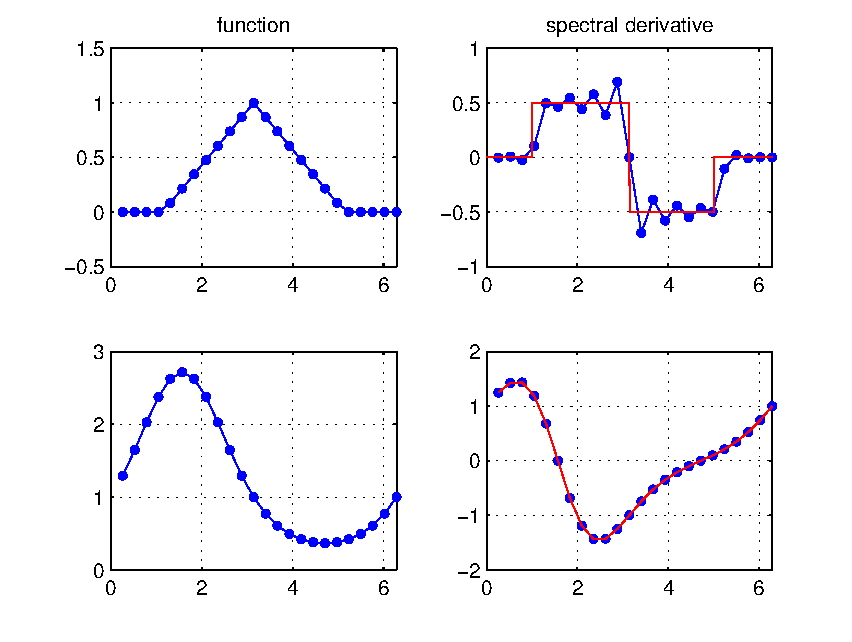
\includegraphics[width=\textwidth]{spectral_derivatives.pdf}
\caption{Spectral differentiation of two functions $\max(0,1-|x-\pi|/2)$ (top) and $e^{\sin x}$ (bottom). On the right is the spectral derivative computed with $n=24$. Even as such small $N$, the derivative of $e^{\sin x}$ is very smooth and the error is on the order of $\mathcal{O}(10^{-13})$. The spectral derivative of $\max(0,1-|x-\pi|/2)$ is not as good due to the discontinuity at $x=\pi$.}
\label{spectral_derivatives}
\end{center}
\end{figure}

As we can see in Fig.~\ref{spectral_derivatives} when the original function is sufficiently smooth and periodic, here $g(x)$, the accuracy of the derivative is very good. However, when the function is not smooth, as exhibited in $f(x)$, the accuracy is not very good. Here $g(x)$ is not differentiable at $\pi$ and spectral methods have a difficult time dealing with this. For a complete discussion of the specific smoothness and accuracy is contained in Chapter 4 of \cite{trefethen_spectral}.

In this section, we have focused only on simple one-dimensional examples, but the method easily generalises to arbitrary dimensions. The only technical point is how to compute the $n$-dimensional FFT. (expand this)
%The algorithm to compute the derivatives of a mutlidimensional function $f(x_{1},x_{2},\ldots,x_{n})$
%\begin{enumerate} 
%\item Sample function $f(x_{1},\ldots,x_{n})$ at $N^{n}$ data points to obtain $v_{j_{1},j_{2},\ldots,j_{n}}, j_{i}=1,\ldots,N, i=1,2,\ldots,n$.
%\item Compute, using the $n$-dimesional FFT, $\hat{v}_{k_{1},k_{2},\ldots,k_{n}}$ from $v_{j_{1},\ldots,j_{n}}$.
%\item Multiply $v_{j_{1},\ldots,j_{n}}$ by $(ik_{1})^{m_{1}}(ik_{2})^{m_{2}}\ldots(ik_{n})^{m_{n}}$ to compute the derivative in the desired variables and orders.
%\item Invert the result using the $n$-dimensional IFFT. 
%\end{enumerate}
\section{Dealiasing} 
In the previous section we demonstrated that spectral differentiation can produce very accurate results in only $\mathcal{O}(N\log N)$ operations. However, we have only considered the spectral derivative of a single function $f(x)$, the question naturally arises about what happens if we have more general expressions, for example advection like terms in the Navier-Stokes equations 
\begin{align}
u\frac{\partial u}{\partial x} + v\frac{\partial u}{\partial y} +w\frac{\partial u}{\partial z}
\end{align}
where we now have a product of a function and a derivative. Such terms are known as a convolution and require a more careful treatment. In this section, we introduce two closely related methods for evaluating expressions of the above form, the spectral method and the pseudospectral method. For this we carefully follow the treatment of Durran \cite{durran}. 

Consider the following general 1D non-linear PDE
\begin{align}
\frac{\partial \psi}{\partial t} + F(\psi) = 0
\end{align}
where $F(\psi)$ is some general nonlinear function. Consider seeking a series expansion of the form
\begin{align}
\psi(x,t)\approx \phi(x,t) = \sum_{k=1}^{N}a_{k}(t)\varphi_{k}(x)
\end{align}
where $\varphi_{k}$ are basis functions around which we are interested in expanding the solution. Some examples of such functions might be complex exponentials, Bessel functions, or spherical harmonics, however, in general,  we will not be able to find the eigenfunctions that provide the natural basis to seek a series expansion. Without the proper basis functions, it is clear that the approximate solution will never exactly solve the original PDE and we have to determine a way to minimise the error. For many problems, there is often some degree of symmetry so choosing a certain basis makes sense. For example, for a problem within a periodic box, it makes sense to choose complex exponentials as a basis; or if the problem is based on a sphere, spherical harmonics are a natural choice. Thus, we are interested in not finding the correct $\varphi_{k}$ but instead focus picking a basis and appropriately choosing $a_{k}(t)$ to minimise the residual, 
\begin{align}
R(\phi) = \frac{\partial \phi}{\partial t} + F(\phi),
\end{align}
in some way.  

\subsection{Spectral Method}
How we choose to evaluate this error leads to different methods of solving the problem. Right now we consider the so-called "spectral method" which is a special case of a very general technique called Galerkin approximation.  The spectral method requires the residual be orthogonal to the basis functions $\varphi_{k}$, i.e.
\begin{align}
\int_{S}R(\phi(x))\varphi_{k}(x)dx = 0 \qquad k=1,\ldots,N.
\end{align}
For the special case of the spectral method, we require that the basis functions be orthogonal. Other basis functions that are not orthogonal but satisfy other constraints, such support over very small areas, lead to a different approximation known as the finite element method\cite{durran}.

By requiring the above integral to be minimised, it can be shown\cite{durran} that the resulting system of ODEs for the above is
\begin{align}
\frac{d a_{k}}{dt} = -\frac{1}{M_{k,k}}\int_{S}\left[F\left(\sum_{n=1}^{N}a_{n}\varphi_{n}\right)\varphi_{k}\right]dx \qquad k=1,\ldots,N
\end{align}
where $M_{k,k}=\langle \varphi_{k},\varphi_{k}\rangle$. For our work, we are interested in a specific case of basis functions, $\varphi_{k}(x)=e^{ikx}$ and the inner product to be the standard inner product for complex functions
\begin{align}
\int_{S}g(x)h^{*}(x)dx=0 
\end{align}

To demonstrate the above formulation, we use the spectral method to solve the 1D advection equation with variable windspeed,
\begin{align}
\frac{\partial\phi}{\partial t} + c(x,t)\frac{\partial \phi}{\partial x} =0, F(\phi) = c(x,t)\frac{\partial \phi}{\partial x}.
\end{align}
We now expand out $\phi(x,t)$ as the sum of $N=2K+1$ Fourier modes, where here we are now letting $N$ be an odd number in contrast to the previous section where $N$ was even. This is chosen because it simplifies the formulas, however the results hold for even $N$ as well, but with some slight alterations to the algebra. Expanding
\begin{align}
\phi(x_{j},t)= \sum_{n=K}^{K}a_{n}(t)e^{inx_{j}},
\end{align}
and plugging this into the above yields
\begin{align}
\frac{d a_{k}}{dt} = -\frac{i}{2\pi}\sum_{n=-K}^{K}na_{n}\int_{-\pi}^{\pi}c(x,t)e^{i(n-k)x}dx \qquad k=-K,\ldots,K.
\end{align}
Expanding out $c(x,t)$ as a Fourier series we obtain
\begin{align} 
\frac{d a_{k}}{dt} = -\frac{i}{2\pi}\sum_{n=-K}^{K}\sum_{m=-K}^{K}na_{n}c_{m}\int_{-\pi}^{\pi}e^{i(n+m-k)x}dx \qquad k=-K,\ldots,K
\end{align}
and upon using the orthogonality of the integral, we obtain
\begin{align}
\frac{da_{k}}{dt} = -\sum_{\substack{m+n=k\\ |m|,|n|\le K}} inc_{m}a_{n}
\end{align}
where we require that $n+m=k$ and $|n|,|m|\le K$. If we want to evaluated this sum directly, we would need to evaluate $\mathcal{O}(K^{2})$ operations due to the double sum required to evaluate the convolution. Historically, this was a barrier for spectral methods because even though they provided accurate results, this $\mathcal{O}(K^{2})$ bottleneck did not allow for larger numerical simulations, where $\mathcal{O}(K)$ finite differences method could. (ref)

In order to get around this bottleneck, we can turn the $\mathcal{O}(K^{2})$ to $\mathcal{O}(K\log K)$ using the FFT. The general idea is as follows: transform the Fourier coefficients to real space in $\mathcal{O}(K\log K)$, multiply the two terms together at each grid point in $\mathcal{O}(K)$, and transform back to Fourier space in $\mathcal{O}(K\log K)$. The resulting algorithm is $\mathcal{O}(K\log K)$. However, if we were to implement this naively, errors would arise, due to the phenomena of aliasing. 

At a basic level, aliasing is the result of multiplying two terms grid-pointwise that generate shortwaves that can be aliased into long waves. This arises in the spectral method when we compute the product of two Fourier coefficients. A very similar, but exaggerated example, is known as the wagon wheel effect and can illustrate the general idea of short waves being interpreted as long waves. (Wikipedia) The wagon wheel effect arises when an object appears to be stationary but is really moving. For example, imagine a camera that takes a picture every second of a turbine, but the turbine is moving at 10 revolutions per second. For someone looking at the shots from the camera, they would claim the turbine isn't moving. If the turbine is moving slightly faster, say 10.1 revolutions per second, the camera would show that the turbine is moving, albeit rather slowly. If it were moving slightly slower, say 9.9 revolutions per second, the camera would show the turbine moving backwards. Thus one would interpret the turbine as moving very slowly in either case and thus conclude that it must have a very slow period, or long wavelength. In actuality, the period is much more rapid and the wavelength of one revolution is much shorter.  
\begin{figure}
\begin{center}
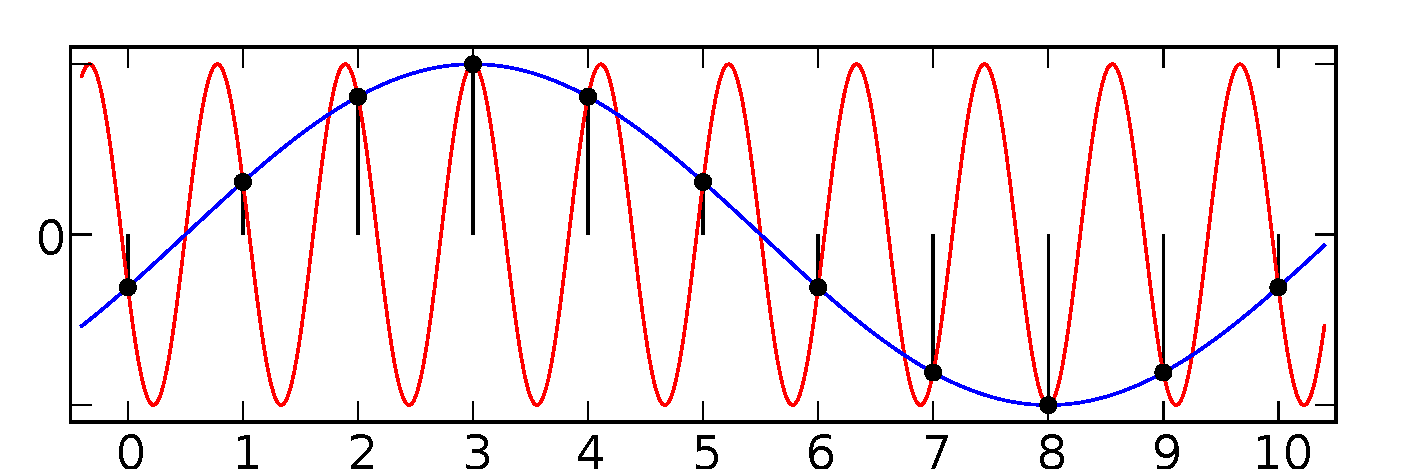
\includegraphics[width=\textwidth]{aliassine.pdf}
\caption{Different sine curves that fit the same set of data points. This is an example of aliasing. Source http://en.wikipedia.org/wiki/File:AliasingSines.svg}
\label{aliassine}
\end{center}
\end{figure}

Mathematically, we can see a similar phenomena by sampling a sine wave. Consider Figure~\ref{aliassine} which has 11 points. The short wavelength red sine curve samples these points with a short wavelength while a longer wavelength blue curve also samples, despite being non-existent in the actual data. The goal is to minimise this effect. 

To illustrate this consider two functions $f(x),g(x)$ we want to compute the Fourier coefficients so that
\begin{align}
f(x)g(x) = \sum_{m=-K}^{K} p_{k}e^{ikx}
\end{align}
and we can expand $f(x),g(x)$ as Fourier series
\begin{align}
f(x) = \sum_{m=-K}^{K}a_{m}e^{imx}, \qquad g(x) = \sum_{n=-K}^{K}b_{n}e^{inx}
\end{align}
The above algorithm states that we convert the Fourier coefficients $a_{m},b_{n}$ to real space and multiply. Suppose that in real space the spacing between the grid points is
\begin{align}
x_{j} = \frac{2\pi j}{2N+1}
\end{align}
where we let $2N+1$ denotes the total number of grid points. We have chosen this notation so to make explicit that each wavenumber should have a corresponding grid point on the real grid. 

(note beginning here I want to rewrite this section)
How do we choose $N$? Naively, it seems logical to set that $N=K$ so that both real and Fourier space have the same number of co-efficients. This naive choice leads to aliasing error and instead we must choose $N>K$ to avoid this aliasing error. To get intuition for why, aliasing error arises when two poorly resolved waves are multiplied together and produce a longer wavelength wave, as discussed above in Figure~\ref{aliassine}. We can avoid this if all short wavelengths are resolved properly.

To find the optimal value of $N$, consider multiplying the two largest wavenumber in Fourier space, here $2K$. The largest possible wavenumbers, which correspond to the smallest scales, can be produced when multiplying two waves is $K+K$, recalling that multiplication of waves is addition of the wavenumbers. The largest possible resolvable wave in the real space grid is $\pi/\dx=N+1/2$. Here we can explicitly see what happens if $K=N$. The $2K=2N$ waves would not be resolved properly because the largest possible wavenumber to be resolved is only $N$. An obvious choice to fix this is to choose $N=2K$ and thus we could resolve all possible wavenumbers. However this choice is too loose a bound since it would imply that for every simulation, we would require twice as many grid space coefficients as Fourier coefficients. It is possible to do better. 

To do better, consider which wavenumber the $2K$ would be dealiased into, which will be $2K-2\pi/\dx$ thus..  
\begin{align}
K<|2K- \frac{2\pi}{\dx}|
\end{align}
and upon subbing in $\dx$ we find that 
\begin{align}
N > \frac{3}{2}K - 1
\end{align}
(end section to rewrite)

There is an alternative way to get at the same result. Consider the discrete Fourier transform of the product $f(x)g(x)$
\begin{align}
p_{k} = \frac{1}{2N+1}\sum_{j=1}^{2N+1}f(x_{j})g(x_{j})e^{-ikx_{j}},
\end{align}
and now plug in the 
\begin{align}
f(x) = \sum_{m=-N}^{N}a_{m}e^{imx}, \qquad g(x) = \sum_{n=-N}^{N}b_{n}e^{inx},
\end{align}
where we have replaced $K$ with $N$ where $N>K$. This is the same expansion as before but we have set $a_{l},b_{l}=0$ if $K < |l|\le N$. Plugging these into the above yields
\begin{align}
p_{k} = \frac{1}{2N+1}\sum_{m=-N}^{N}\sum_{n=-N}^{N}\sum_{j=1}^{2N+1}a_{m}b_{n}e^{i(m+n-k)x_{j}}.
\end{align}
Recalling that $x_{j} = 2\pi j/(2N+1)$ the inner summation is
\begin{align}
\sum_{j=1}^{2N+1}e^{i(m+n-k)x_{j}} =  \begin{cases}
1 & m+n-k =0\\
1 & m+n-k =2N+1\\
1 & m+n-k =-(2N+1)\\
0 & \text{otherwise}
\end{cases}
\end{align}
which is a restatement of the well known orthogonality condition \cite{durran}. Thus we can break up the above summation into three cases, $m+n=k, m+n=k\pm(2N+1)$ which gives
\begin{align}
p_{k} = \sum_{\substack{m+n=k\\ |m|,|n|\le N}}a_{m}b_{n}+  \sum_{\substack{m+n=k+2N+1\\ |m|,|n|\le N}}a_{m}b_{n}+ \sum_{\substack{m+n=k-2N-1\\ |m|,|n|\le N}}a_{m}b_{n}.
\end{align}
Note the similarity with the result from the spectral method, which is identical to summation encountered in the spectral method, recalling that the coefficients are zero for values greater then $K$. The aliasing error arises from the second two terms. We want to eliminate this error so we have to decide how to choose $N$ to eliminate this term. We consider the first aliasing error term. We have that if $m,n>K$ then $a_{m}b_{n}=0$. It follows that $m+n>2K$ this term will vanish, i.e. $m+n=k+2N+1>2K$ for all $k=-K,\ldots,K$. Thus we want to consider $k=-K$ since this is the smallest possible value of this summation, i.e. $-K+2N+1>2K$. Rearranging this yields $N>(3K-1)/2$ as before. An identical argument gives the same result for the other aliasing term. 

This dealiasing rule is known as the ``two-thirds rule" and will completely eliminate aliasing effects. The above algorithm tells us how to choose $N$ given $K$, however in many applications we typically work the other way around, choosing $N$ and limiting $K$. We now can now write down the algorithm for evaluating the following term $c(x)\partial\phi/\partial x$ in Fourier space, when we are initially only given $M$ samples: 
\begin{itemize}
\item Sample $c(x),\phi(x,t)$ at $M$ points.
\item Compute the Fourier coefficients of $c(x),\phi(x,t)$ using the FFT yielding $M$ Fourier coefficients $a_{i},b_{j}$ respectively.
\item Evaluate the spectral derivative of $\phi$ by multiplying the coefficients by $ik$, i.e $a_{l}=ika_{l}$.
\item Modify the Fourier coefficients so the top $1/3$ are zero. 
\item Take the IFFT back to real space.
\item Multiply the real space coefficients gridwise.
\item Take the FFT of this product.
\end{itemize}
This procedure will allow us to evaluate the Navier-Stokes equations in Fourier space by evaluating convolution terms by multiplying fields in real space and to eliminate numerical error. In the next section, we provide a simple example that illustrates this method in practice.

\subsection{Pseudospectral Method}
We have just been focusing on eliminating the aliasing error at the cost of eliminating some Fourier modes which can be achieved by taking $N>3K/2$. A very closely related, but different method is known as, somewhat confusingly, as the pseudospectral method is an alternative way to evaluate the above equations. In this case, instead of enforcing that the residual is orthogonal to the basis functions, we instead choose a collocation method, i.e.
\begin{align}
R(\phi(j\dx)) = 0,
\end{align}
where we enforce that the coefficients satisfying the equation at each grid point. Let us now expand $\phi(x,t),c(x,t)$ are Fourier series
\begin{align}
\phi(x,t) = \sum_{n=-K}^{K}a_{n}e^{inx}, \qquad c(x,t) = \sum_{m=-K}^{K}c_{m}e^{imx}.
\end{align}
Substituting into the test equation and enforcing the collocation requirement yields
\begin{align}
\sum_{n=-K}^{K}\frac{da_{n}}{dt}e^{inx_{j}} + \sum_{m=-K}^{K}c_{m}e^{imx_{j}}\sum_{n=-K}^{K}ina_{n}e^{inx_{j}}=0.
\end{align} 
which we can alternatively write as
\begin{align}
\frac{d\phi_{j}}{dt} + c_{j}\frac{\partial \phi_{j}}{\partial x} = 0,
\end{align}
where we have written
\begin{align}
\phi(x_{j}) = \sum_{n=-K}^{K}a_{n}e^{inx_{j}}, c(x_{j}) = \sum_{n=-K}^{K}c_{n}e^{inx_{j}}, \frac{\partial\phi_{j}}{\partial x} = \sum_{n=-K}^{K}ina_{n}e^{inx_{j}}.
\end{align}
This is the set of equations we want to solve. Thus we now have a way to evaluate using the following algorithm:
\begin{enumerate}
\item Evaluate $\phi(x,t),c(x,t)$ at $M$ points.
\item Compute the spectral derivative of $\phi(x,t)$ using the methods of the previous sections.
\item Multiply all the coefficients gridpoint wise.
\item Timestep the resulting solution.
\end{enumerate} 

\subsection{Spectral vs Psuedospectral}
The equations resulting from the pseudospectral method are actually very similar to the spectral equations except that there is no dealiasing. To why, multiply the above equation by $e^{-ikx_{j}}$ and sum over all $j$ and we will obtain
\begin{align}
\frac{da_{k}}{dt}= -\sum_{\substack{m+n=k\\ |m|,|n|\le K}}inc_{m}a_{n}-\sum_{\substack{m+n=k+2K+1\\ |m|,|n|\le K}}inc_{m}a_{n}- \sum_{\substack{m+n=k-2K-1\\ |m|,|n|\le K}}inc_{m}a_{n}.
\end{align}
For comparison, the spectral method equations are
\begin{align} 
\frac{da_{k}}{dt} = -\sum_{\substack{m+n=k\\ |m|,|n|\le K}} inc_{m}a_{n},
\end{align}
where in both equations $k=-K.\ldots,K$. 

There is a lot of similarity between these two equations but we have to remember that they were derived in two completely different ways. Recall to evaluate the convolution term in the spectral method, we obtained the following equation
\begin{align}
p_{k} = \sum_{\substack{m+n=k\\ |m|,|n|\le N}}a_{m}b_{n}+  \sum_{\substack{m+n=k+2N+1\\ |m|,|n|\le N}}a_{m}b_{n}+ \sum_{\substack{m+n=k-2N-1\\ |m|,|n|\le N}}a_{m}b_{n}.
\end{align}
which has the exact same form as the pseudospectral method but the crucial difference is that the sum is over $N$ and not $K$. If we set $N=K$, which would result in dealiasing error, we would obtain the pseudospectral method. Thus, at a fundamental level, the psuedospectral method is just the spectral method without dealiasing.

In the next section we make the differences explicit with examples and also discuss some results of not dealiasing vs dealiasing. 

\section{Timestepping and Examples}
(introduction to timestepping)

When we choose a time-stepping scheme, the stability of the scheme is important to know. The stability region tells us when we can except our solution to not blow up. To do this we define the amplitude A to be
\begin{align}
A = \frac{\phi_{n+1}}{\phi_{n}}
\end{align}
for the Adams-Bashforth scheme we have 
\begin{align}
\phi_{n+1} = \phi_{n} + \frac{\dt}{2}(3F(\phi_{n}) - F(\phi_{n-1}))
\end{align}
and stability is defined to be 
\begin{align}
|A|^{2} \le 1
\end{align}
since $A$ can potentially be complex. The reasoning from this equation arises from rearranging the above so that $\phi_{n+1}=A\phi_{n}$. If $|A|\le 1$ then the solution is not growing in time. If $|A|>1$ then at each time-step the solution is being multiplied by a number greater then one, hence it is growing. 

To investigate the stability region, the following equation is used\cite{durran}
\begin{align}
\frac{d\phi}{dt} =  (\lambda + i\omega)\phi
\end{align}
where $\lambda,\omega$ are real numbers. To determine the stability region we use the method from Leveque (cite) which gives a stability region of
\begin{align}
z = \frac{2(\xi^{2}-\xi)}{3\xi -1}
\end{align}
where $\xi$ is the unit circle. (Add plot to show stability plus derivation).

In this section we demonstrate the differences between solving PDEs in real space vs Fourier space. Consider the following one dimensional wave equation\cite{trefethen_spectral}
\begin{align}
\frac{\partial u}{\partial t} + c(x)\frac{\partial u}{\partial x} = 0,\qquad c(x)=\frac{1}{5}+\sin^{2}(x-1), \qquad u(x,0)=e^{-100(x-1)^{2}}, x\in[0,2\pi], t>0
\end{align}
where we are solving on a periodic domain. The physical interpretation of this equation is the simple one dimensional advection of a velocity field $u(x,t)$ by the fixed field $c(x)$. To evaluate the advection term, we use a spectral method with 2/3s dealiasing. As discussed in the previous section, there is still non-standard terminology throughout the literature regrading the names of the various methods of using FFTs. Trefethen, for example, calls pseudospectral methods, 'collocation methods'. 

For a time-stepping scheme, we use a second-order Adams-Bashforth\cite{durran} scheme. Re-writing wave-equation as
\begin{align}
\frac{\partial u}{\partial t} = -c(x)\frac{\partial u}{\partial x} = F(u)
\end{align}
which we can write in Fourier space as
\begin{align}
\frac{\partial \hat{u}}{\partial t} = \widehat{-c(x)\frac{\partial u}{\partial x}} = F(\hat{u})
\end{align}
the Adams-Bashforth scheme is
\begin{align}
\hat{u}^{n+1} = \hat{u}^{n} + \frac{\dt}{2}[3F(\hat{u}^{n})-F(\hat{u}^{n-1})]
\end{align}
Since the Adams-Bashforth scheme uses a previous time-step, we will use forward Euler for the first time-step. To evaluate $F(u)$ we will use the spectral differentiation, as discussed above. 

The following code is the MATLAB code for evaluating the advection-diffusion equation with 2/3s deliasing
\begin{verbatim}
%construct the grid and basic parameters
N=128; dx=2*pi/N; x=dx*(1:N);t=0;dt=dx/10;tf=5;nsteps=ceil(tf/dt);
c=0.2+sin(x-1).^2;
%store the wavenumbers
kx=[0:N/2-1 0 -N/2+1:-1];
%define cut to cut out the highest Fourier modes
cut=ones(1,N); ksq=kx.*kx;
%cut out the Fourier co-efficients according to dealiasing 
%because of wavenumber ordering cut out (most negative wave numbers start
%at N/2) e.g. (2/3)*(N/2) : (N/2+(1/3)(N/2) for 2/3s
cut(ceil(dealias_coeff*N/2):(N/2+ceil((1-dealias_coeff)*N/2))+1)=0;
%initial condition
u=exp(-100*(x-1).^2);uhat=fft(u);
%do initial timestep using Euler
Fold=-fft(c.*real(ifft(1i*cut.*kx.*uhat)));
uhat=(uhat+dt*Fold); 

%do Adams Bashforth
for i=1:nsteps
    F=-fft(c.*real(ifft(1i*cut.*kx.*uhat)));
    uhat=uhat+1.5*dt*F-0.5*dt*Fold;
    Fold=F;
end
\end{verbatim}
In the above code the line \texttt{ifft(1i*cut.*kx*uhat)} evalutes the spectral derivative of the velocity field and adds in the dealiasing by cutting out the top 1/3 of the Fourier coefficients. Note that MATLAB stores the wavenumbers \texttt{kx=[0:N/2-1 0 -N/2+1:-1]} and thus to zero out the correct coefficients requires some clever index manipulation. 
\begin{figure}
\begin{center}
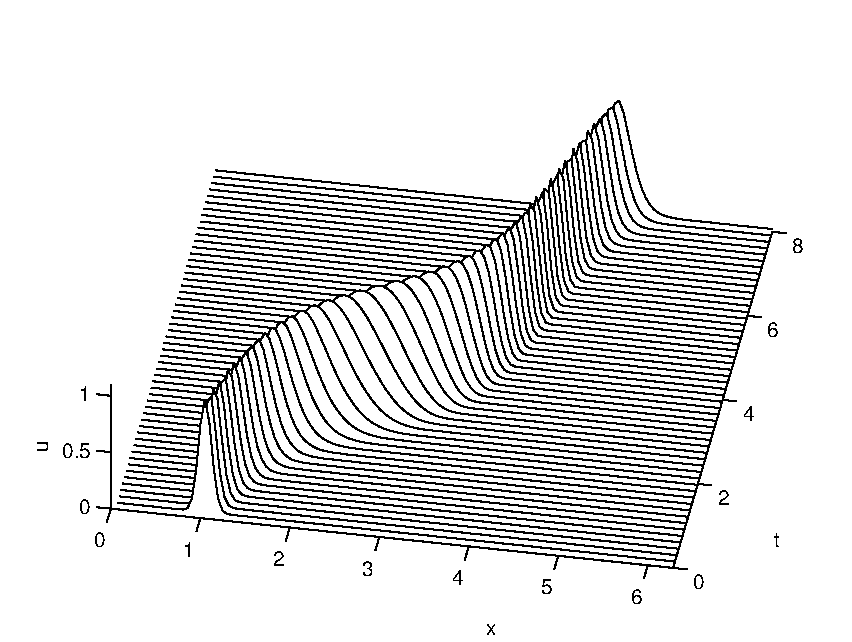
\includegraphics[width=\textwidth]{spectral_example.pdf}
\caption{Spectral solution to the advection equation with variable windspeed. Figure is a reproduced version of Output 6 of Trefethen \cite{trefethen_spectral}}
\label{spectral_example}
\end{center}
\end{figure}
Fig.~\ref{spectral_example} demonstrates the solution to the above advection equation using spectral methods. As can be observed, the solution is very smooth and evolves very clearly for only $N=128$.


To illustrate the differences between the spectral and pseudospectral method, or 2/3s dealiasing vs no dealiasing, we solve the viscous Burger's equation
\begin{align}
\frac{\partial \phi}{\partial t} + \phi\frac{\partial \phi}{\partial x} = \nu \frac{\partial^{2}\phi}{\partial x^{2}}
\end{align}
with a Gaussian initial condition. Instead of using the Adams-Bashforth scheme, we use an RK4 to eliminate numerical instabilities that result when the Adams-Bashforth scheme was used. Indeed, the actual scheme is irrelevant to the results and what it is important to illustrate the energy conversation of the spectral method while the pseudospectral method does not. This is because the spectral method conservees energy while the psuedospectral method does not. 

%In Panel A we have spectral methods and we can see that the total energy is constant while with the pseudospectral in Panel B diverges. 

Discuss dealiasing of linear and nonlinear code as well. Show plots. 
\section{Navier-Stokes in Fourier Space}
\subsection{Fourier Transformed Navier-Stokes}
We now turn to the formulation of the Navier-Stokes equations in a Fourier domain. The Fourier domain provides a convenient formulation to analyse the underlying mechanisms of turbulence, as we shall see. Recall that in the Fourier domain, derivatives become multiplication of wavenumbers which converts the spatial parts of the Navier-Stokes equations into algebraic equations. 

To demonstrate the formulation in Fourier space, let us cast the standard Navier-Stokes equations into Fourier space. 
\begin{align}
\frac{\partial \textbf{u}}{\partial t} + \textbf{u}\cdot\nabla\textbf{u} = -\frac{1}{\rho_{0}}\nabla p + \nu\nabla^{2}\textbf{u}, \qquad \nabla\cdot\textbf{u}=0
\end{align}
Taking the Fourier transform of the above equation is straight-forward for all terms except the advection term $\textbf{u}\cdot\nabla\textbf{u}$, which we postpone for now.

In Fourier space, we can also exploit the following observation to eliminate the pressure term, thus saving the need to solve a Poisson equation at each time-step. The incompressibility condition becomes $\textbf{k}\cdot\hat{\textbf{u}}(\textbf{k},t)=0$ in Fourier space. Geometrically, this means that the vectors $\textbf{k}$ and $\hat{\textbf{u}}$ are orthogonal. To see this define a $\textbf{k}$-plane and a $\hat{\textbf{u}}$-plane. The defining equation of a plane is $ax+by+cz=d$ with the normal vector $\textbf{n}=(a,b,c)$. Here the normal vectors are $\textbf{k}$ and $\hat{\textbf{u}}$. Thus if the normal vectors are orthogonal, the planes are orthogonal.

This realisation tells us that vectors that are proportional to \uhatm are orthogonal to vectors that are proportional to \kvecm. Thus writing out the Navier-Stokes equations
\begin{align}
\frac{\partial \uhat}{\partial t} + \mathcal{F}(\textbf{u}\cdot\nabla\textbf{u}) = -\frac{1}{\rho_{0}} \kvec\hat{p} - \nu k^{2}\uhat\label{NS_fourier_1},
\end{align}
take the dot product with \kvecm and using the orthogonality condition we obtain
\begin{align}
\kvec\cdot\mathcal{F}(\textbf{u}\cdot\nabla\textbf{u}) + \frac{1}{\rho_{0}}k^{2}\hat{p}=0\label{pressure_fourier_1}.
\end{align}
Isolating for pressure and substituting back into (\ref{NS_fourier_1}) we obtain
\begin{align}
\frac{\partial \uhat}{\partial t} + \mathcal{F}(\textbf{u}\cdot\nabla\textbf{u})(\textbf{1}-\frac{\kvec\kvec}{k^{2}})= - \nu k^{2}\uhat\label{NS_fourier_2}.
\end{align}
This result is unsurprising, since all we have done is take the divergence of the Navier-Stokes equations, which in Fourier space corresponds to taking the dot product with respect to $\kvec$. But using this observation we can avoid the need for solving the pressure altogether because the pressure term is orthogonal to the $\uhat$-plane. But what about the advection term? As can be seen in (\ref{NS_fourier_2}), it has this factor $\textbf{1} - \kvec\kvec/k^{2}$ multiplying it. This term represents a projection into the $\uhat$-plane. The advection term can thought of a vector that is pointing in some direction in-between the planes of $\kvec$ and $\uhat$. By projecting the advection term into the $\uhat$-plane, we would have a set of equations that are independent of the pressure completely.

\subsection{Projection Tensor}
In order to project the Navier-Stokes equations onto the $\uhat$-plane, we define the following projection operator
\begin{align}
\textbf{P}=\textbf{1} - \frac{\kvec\kvec}{k^{2}} \text{ or } P_{ij}(\kvec) = \delta_{ij} - \frac{k_{i}k_{j}}{k^{2}}
\end{align}
where we are using Einstein summation notation \cite{lesieur,wald}. It is straight forward to verify that $P_{ij}P_{jk}=P_{ik}$ or in matrix notation $\textbf{P}^{2}=\textbf{P}$, in other words the projection tensor is idempotent. Idempotence is a defining feature of projection operators \cite{MeyerLinAlg}. It is straightforward to verify that $k_{j}P_{ij}=0$ and $\hat{u}_{j}P_{ij}=\hat{u}_{i}$. These simple observations confirm that the projection tensor projects a vector onto the $\uhat$-plane. 

Applying $P_{ij}$ to (\ref{NS_fourier_1}) we obtain the following 
\begin{align}
\frac{\partial \uhat}{\partial t} + \textbf{P}\mathcal{F}(\textbf{u}\cdot\nabla\textbf{u}) =  -\nu k^{2}\uhat\label{NS_fourier_3}
\end{align}
where $\textbf{P}$ is acting on the Fourier transform of the advection term. In order to compute the Fourier transform of the advection term, we note that 
\begin{align}
\textbf{u}\cdot\nabla\textbf{u} = u_{j}\frac{\partial u_{i}}{\partial x_{j}} = \frac{\partial (u_{i}u_{j})}{\partial x_{j}}
\end{align}
where the incompressibility condition has been used to bring the velocity inside the derivative. Thus we are able to write
\begin{align}
\mathcal{F}(\textbf{u}\cdot\nabla\textbf{u})=ik_{j}\int_{\textbf{p}+\textbf{q}=\kvec}d\kvec\hat{u}_{i}(\textbf{p})\hat{u}_{j}(\textbf{q})
\end{align}
and hence we can finally write out the Navier-Stokes equations in Fourier space as \cite{lesieur}
\begin{align}
\frac{\partial \hat{u}_{i}}{\partial t} + iP_{ij}k_{m}\int_{\textbf{p}+\textbf{q}=\kvec}d\kvec\hat{u}_{j}(\textbf{p})\hat{u}_{m}(\textbf{q})=  -k^{2}\hat{u}_{i}\label{NS_fourier_3}
\end{align}

\subsection{Numerical Formulation of NS in Fourier}
Although we have eliminated the pressure completely, we still have the nonlinear term in the equation. To formulate this problem numerically, we make the following observation that is useful in spectral methods \cite{lesieur,orszag1972}.

Recall the following identity (Kundu, Acheson)
\begin{align}
\textbf{u}\cdot\nabla\textbf{u} = \bm{\omega}\times \textbf{u} - \frac{1}{2}\nabla \textbf{u}^{2}
\end{align}
When we apply the projection operator $\textbf{P}$ to the above equation, the $\nabla \textbf{u}^{2}$ term will vanish since it is orthogonal to the $\uhat$-plane. For the cross product between the vorticity and velocity, we use the methods discussed above from dealiasing. Thus to evaluate the cross product term, we assume we have the Fourier transform of the vorticity and velocity $\hat{\bm{\omega}},\uhat$ and re-write the cross product term as
\begin{align}
\mathcal{F}(\bm{\omega}\times \textbf{u}) = \mathcal{F}(\mathcal{F}^{-1}(\hat{\bm{\omega}})\times\mathcal{F}^{-1}(\uhat))
\end{align}
Using this result we can reformulate the Navier-Stokes equations into a form to be solved numerically using a spectral method
\begin{align}
\frac{\partial \uhat}{\partial t} = \textbf{P}(\kvec)\mathcal{F}(\mathcal{F}^{-1}(\hat{\bm{\omega}})\times\mathcal{F}^{-1}(\uhat))-k^{2}\uhat
\end{align}
where the $\mathcal{F},\mathcal{F}^{-1}$ can be evaluated by FFTs, as discussed above.

This reformulation of the Navier-Stokes equations into Fourier space simplifies numerical calculations immensely and provides many advantages over the real space formulation. The absence of the pressure term means that there is no Poisson equation to be solved at each time-step for the pressure. If one did want the pressure, one can solve (\ref{pressure_fourier_1}) for $\hat{p}$. In addition there is no need to enforce a divergence free solution\footnote{Except possibly at the initial time step and periodically during a simulation due to numerical errors.} as the equations are formulated by definition to satisfy divergence free condition. The only additional technical difficulty is evaluating the vorticity, but this can easily be handled because of the simple structure of the curl. 

\subsection{Integrating Factor}
Another advantage of the Fourier formulation is the ability to exactly integrate the diffusion term. Let us denote the advective projective term as $F(\hat{u})$ and we have
\begin{align}
\frac{\partial \uhat}{\partial t} + \nu k^{2}\uhat = F(\uhat) 
\end{align}
where the left-hand side has been explicitly written out. Written in this form, the common trick of writing a product as a derivative is observed since
\begin{align}
 \frac{\partial \uhat}{\partial t} + \nu k^{2}\uhat= e^{-\nu k^{2}t}\frac{\partial }{\partial t}(\uhat e^{\nu k^{2}t})
\end{align}
Thus we can re-write the Navier-Stokes equations as 
\begin{align}
\frac{\partial }{\partial t}(\uhat e^{\nu k^{2}t})= e^{\nu k^{2}t}F(\uhat) 
\end{align}
For notational convenience, let us write $g(t) = e^{\nu k^{2}t}$ and the note the following trivial identities
\begin{align}
g(t\pm\dt) = g(t)g(\pm\dt),\qquad g(0) = 1, \qquad g(t)^{-1} = g(-t).\label{int_fact_ident}
\end{align}
With this notation the Navier-Stokes equations become
\begin{align}
\frac{\partial (\uhat g(t))}{\partial t} = g(t)F(\uhat).
\end{align}
 Now let us solve the above system using an Adams-Bashforth 2nd order time-stepping scheme. Initially we obtain
\begin{align}
\uhat^{n+1}g(t_{n}+\dt) = \uhat^{n}g(t_{n}) + \frac{3}{2}\dt g(t_{n})F(\uhat^{n}) - \frac{1}{2}\dt g(t_{n-1})F(\uhat^{n-1}).
\end{align}
Using the identities in (\ref{int_fact_ident}) the scheme reduces to
\begin{align}
\uhat^{n+1} = g(-\dt)\uhat^{n} + \frac{3}{2}\dt g(-\dt)F(\uhat^{n}) - \frac{1}{2}\dt g(-2\dt)F(\uhat^{n-1}),
\end{align}
and the diffusion term has been reduced to a multiplication by a constant factor $g(-\alpha\dt)$.

\subsection{Hyperviscosity}
Hyperviscosity is a method of simulating higher Reynolds number flow by replacing the diffusion term with higher derivatives. In the Fourier picture, the diffusion term is $-\nu k^{2}\uhat$. The diffusion timescale $\tau_{d}$ is given by the inverse of $\nu k^{2}$. This implies that the longest wavelengths (smallest $k$) have very long diffusive time-scales while the shortest wavelengths (larger $k$) have very short diffusive time-scales. This picture makes physical sense since viscosity plays a role at the very small scales. As we decrease the viscosity $\nu$ the time-scales of all scales increases. Numerically, if we decrease the viscosity too much, resolution of the smallest scales becomes critical and can lead to unwanted grid-scale effects. Thus, in order to decrease the diffusive time-scales of all wavelengths we can instead vary the power of the wave number. For example, going from $k^{2}$ to $k^{4}$, and adjusting the coefficient accordingly, the time-scales of the various wavelengths would decrease. This is illustrated in Fig~\ref{hyper_vis_example}.

\begin{figure}
\begin{center}
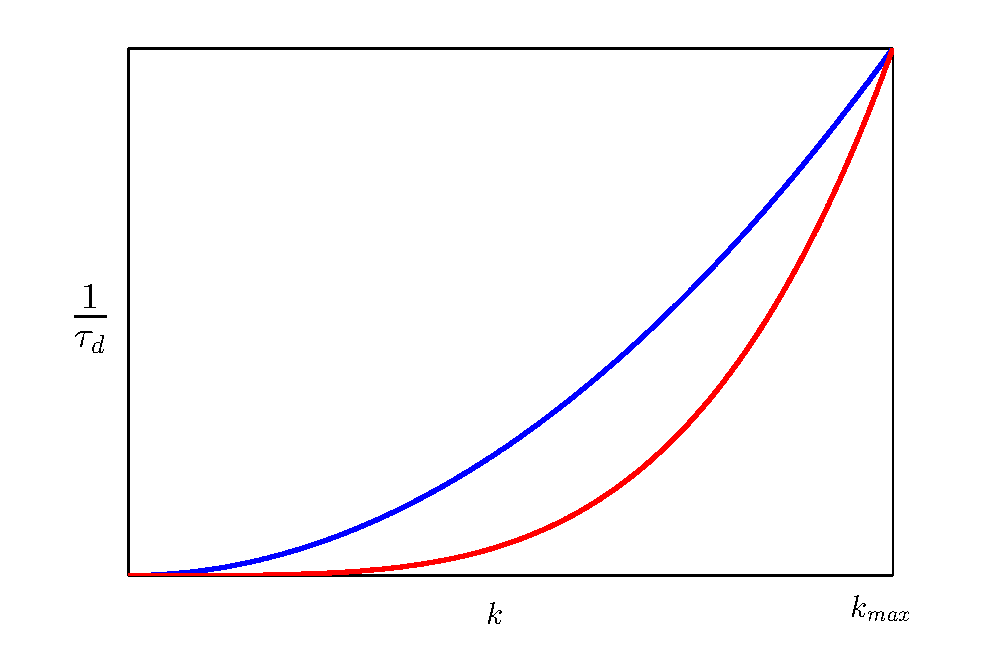
\includegraphics[width=\textwidth]{hyper_vis_example.pdf}
\caption{The inverse diffusion times, $1/\tau_{d}$, of the wavenumbers for the regular viscosity, blue, and the hyperviscosity case, red. The hyperviscosity inverse diffusion times are lower then the regular viscosity case, corresponding to longer diffusion times. This has the effect of simulating larger Reynolds numbers. Note that at $k_{max}$ the two cases coincide.}
\label{hyper_vis_example}
\end{center}
\end{figure}
In general we consider $k$ to be an even number, since this corresponds to even derivatives, however as long as we correctly choose the co-efficient in front of the $k^{n}$ to be $-1$, we can obtain different degrees of diffusion. But if we allow this, odd powers of $k$ no longer correspond to odd derivatives as we will be off by a factor of $i$ and we cannot interpret these derivatives as dispersive terms.

In order to do encorporate hyperviscosity numerically, we scale by the maximum wavenumber $k_{max}$. We want the diffusive timescales of the smallest scales to be the same for both the regular viscosity and the hyperviscosity. That is we want 
\begin{align}
\nu k_{max}^{2} = \nu_{i}k_{max}^{i},
\end{align}
where $i$ is an even integer. Solving for $\nu_{i}$ then gives the following replacement
\begin{align}
\nu k^{2} \Rightarrow \nu k_{max}^{2-i}k^{i}.
\end{align}
Throughout this thesis, we will use $i=4$. 

\subsection{Concluding Remarks (rename)}
Although we have done all our manipulations in Fourier space, we could have equally well formulated the above equations in real space. The idea of projecting the velocity field onto the $\uhat$-plane is motivated by the Helmholtz decomposition. This decomposition states, for any $C^{2}$ vector field in a bounded region of $\mathbb{R}^{3}$, we can decompose the vector field into a divergence-free and curl-free component. The divergence free part corresponds to taking the divergence of the Navier-Stokes equations which would yield the Poisson equation for the pressure. Taking the curl of the Navier-Stokes equation - which we define to be the vorticity - would yield the vorticity equation which does not have a pressure term.


\section{Numerical Scheme for Linear and Nonlinear Boussinesq Equations}
\subsection{Linear Boussinesq Equations Scheme}
We now write the fields as a basic state plus perturbations, denoted by $\sim$. Ignoring the viscous diffusion of the basic state \cite{drazinreid} (add tests from nonlinear code here to justify this point) and neglecting products of the perturbations, we obtain the following set of linear equations for the perturbations
\begin{align}
\frac{\partial \tilde{\bm{u}}}{\partial t} + \omega_{z0}\hat{\bm{e}}_{z}\times \tilde{\bm{u}}+\tilde{\boldsymbol{\omega}}\times \bm{u}_{h0} = -\nabla(\tilde{p}+\bm{u}_{h0} \cdot \tilde{\bm{u}}) - \tilde{\rho}'\hat{\bm{e}}_{z} + \frac{1}{Re}\nabla^{2}\tilde{\bm{u}},\label{nsl1}\\
\nabla\cdot\tilde{\bm{u}}=0,\\
\frac{\partial \tilde{\rho}'}{\partial t} + \bm{u}_{h0}\cdot \nabla_{h}\tilde{\rho}'-\frac{1}{F_{h}^{2}}\tilde{w} = \frac{1}{ScRe}\nabla^{2}\tilde{\rho}',\label{nsl3}
\end{align}
where $\tilde{\boldsymbol{\omega}}=\nabla \times \tilde{\bm{u}}$.

As stated above, the Lamb-Chaplygin dipole is oriented vertically. As a result we can separate the perturbation into the vertical and horizontal directions as 
\begin{align} 
[\tilde{\bm{u}},\tilde{p},\tilde{\rho}'](x,y,z,t) = [\bm{u},p,\rho'](x,y,t)e^{ik_{z}z} + \text{c.c.},
\end{align}
where c.c. is the complex conjugate. From here we can now take the 2D Fourier transform and and recall the projection operator $\textbf{P}(\textbf{k})$, with components $P_{ij}(\textbf{k})=\delta_{ij} - k_{i}k_{j}/k^{2}$ to eliminate pressure, to obtain a set of equations for the Fourier coefficients 
\begin{align}
\frac{\partial \hat{\bm{u}}}{\partial t} = \textbf{P}(\textbf{k})[\widehat{\bm{u}\times \omega_{z0}\hat{\bm{e}}_{z}} + \widehat{\bm{u}_{h0}\times\bm{\omega}}-\hat{\rho}'\hat{\bm{e}}_{z}] - \frac{k^{2}}{Re}\hat{\bm{u}},\label{solve1}\\
\frac{\partial\hat{\rho}'}{\partial t} = -i\bm{k}_{h}\cdot\widehat{\bm{u}_{h0}\rho'} + \frac{1}{F_{h}^{2}}\hat{w}- \frac{k^{2}}{ScRe}\hat{\rho}',\label{solve2}
\end{align}
where $k_{z},Re,Sc,F_{h}$ are input parameters, $\bm{k}_{h}=(k_{x},k_{y})$ is the horizontal wavenumber and $k^{2}=k_{x}^{2}+k_{y}^{2}+k_{z}^{2}$ is the total wavenumber. 

To numerically solve (\ref{solve1}) and (\ref{solve2}), we use a spectral transform method to evaluate derivatives, with 2/3-rule de-aliasing and second order Adams-Bashforth for time-stepping. Each simulation was initialised with a random field and integrated over an $N\times N$ grid for 100 time units to determine the behaviour of the fastest growing mode. After several time units, the leading eigenmodes for $\bm{u},\rho$ behave exponentially (e.g. Billant and Chomaz \cite{bc2000c})
\begin{align}
\bm{u},\rho \propto C(x,y)e^{\sigma t},
\end{align}
and we can obtain the largest growth rate by the formula
\begin{align}
\sigma = \lim_{t\rightarrow\infty}\frac{1}{2}\frac{d\ln E}{dt}\label{sigma1},
\end{align}
where $\sigma$ is the real growth rate of the mode and $E$ is the kinetic energy $\frac{1}{2}(u^{2}+v^{2}+w^{2})$. This follows directly from the exponential behaviour of the leading eigenmode. The energy behaves as
\begin{align}
E \sim \frac{3}{2}C(x,y)^{2}e^{2\sigma t} \Rightarrow \ln E = \ln(3C^{2}/2) + 2\sigma t
\end{align}
and upon taking the time derivative of both sides yields the desired result. To obtain the energy, we use Parseval's theorem which relates the real space energy to the sum of the squares of the Fourier coefficients. Thus the total kinetic energy (domain averaged?) is obtained by summing the squares of the Fourier transform of the velocities over all wavenumbers. 

To evaluate $\sigma$, we compute the average value of the growth rate from the time series. Initially, there is transient behaviour where the various modes are all growing and none dominant (add figure of time series). After $t=20$, after the initial transient behaviour has died out and the leading mode dominants in all the cases observed. In the case of an oscillatory growth rate, as considered in \cite{bc1999}, we drop the assumption that $\sigma$ is real and instead compute the growth rate from
\begin{align}
\sigma_{r} = \lim_{t\rightarrow \infty} \frac{1}{2T}\ln\left(\frac{E(t+T)}{E(t)}\right)\label{sigma2},
\end{align}
where $T$ is the period of the oscillatory mode. (add figure of oscillatory growth rates). The imaginary growth rate is given as $\sigma_{i}=2\pi/T$. As above, we compute $\sigma$ from the time series beginning at $t=20$, however we first measure the period $T$ from roughly 10 oscillations, and then compute the average.  

For our simulations a grid size of $L=9$ with $N=512$ points was used with timestep $\Delta t=0.000950$ for $F_{h}=0.2,Re=2000,5000,10000$ and $\Delta t=0.000375$ for all the other simulations. Unlike Billant and Chomaz\cite{bc2000c} we did not restart each simulation with the previous eigenmode because we used a parallel approach for evaluating multiple $k_{z}$ simultaneously. We investigate a range of Froude and Reynolds number and a wide range of $k_{z}$ from $1$ to $200$ depending on the Froude and Reynolds number. This wavenumber range incorporates the scale of the zigzag instability down to the viscous damping scale. We take $Sc=1$ for all simulations.  

To simulate higher Reynolds number, we use a hyperviscosity operator. The $\nu\nabla^{2}$ diffusion term is replaced with a $\nu_{4}\nabla^{4}$ diffusion term. The $\nu_{4}$ coefficient is chosen so that $\nu k_{max}^{2} = \nu_{4}k_{max}^{4}$, where $k$ is the maximum dealiased horizontal wave number. This allows us to define the hyperviscosity Reynolds number $Re_{h}=Re k_{max}^{2}$. The hyperviscosity simulation was run with $F_{h}=0.1$ and $Re=20000$ with the same numerical parameters as the regular viscosity simulation.

\subsection{Nonlinear Boussinesq Scheme}

That will go here when nonlinear chapter is written. 
